
\section{Постановка задачи}

Задан линейный стационарный объект
\[
\dot{\bm x}=A\bm x+\bm b u
\]

Матрицы системы и параметры критерия качества имеют вид
\[
A=\begin{pmatrix}
0&1\\
-2&9
\end{pmatrix},
\qquad
\bm b=\begin{pmatrix}4\\8\end{pmatrix},
\qquad
Q=\begin{pmatrix}3&0\\0&2\end{pmatrix},
\qquad r=1
\]

Критерий качества
\[
J=\int_0^\infty
\left(\bm x^{T}(\tau)Q\bm x(\tau)
+ru^2(\tau)\right)\,d\tau
\]

Оптимальный регулятор ищем в виде
\[
u^*=-K\bm x
\]

\section{Расчёт оптимального регулятора}

Коэффициенты регулятора определяются из алгебраического
уравнения Риккати
\[
A^{T}P+PA+Q
-P\bm b r^{-1}\bm b^{T}P=0
\]

Матрицу $P$ представим в симметричном виде
\[
P=\begin{pmatrix}
p_{11}&p_{12}\\
p_{12}&p_{22}
\end{pmatrix}
\]

Вычислим слагаемые уравнения Риккати
\[
\begin{aligned}
A^{T}P
&=
\begin{pmatrix}0&-2\\1&9\end{pmatrix}
\begin{pmatrix}p_{11}&p_{12}\\p_{12}&p_{22}\end{pmatrix}
\\[2mm]
&=
\begin{pmatrix}
-2p_{12}&-2p_{22}\\
p_{11}+9p_{12}&p_{12}+9p_{22}
\end{pmatrix}
\end{aligned}
\]

\[
\begin{aligned}
PA
&=
\begin{pmatrix}p_{11}&p_{12}\\p_{12}&p_{22}\end{pmatrix}
\begin{pmatrix}0&1\\-2&9\end{pmatrix}
\\[2mm]
&=
\begin{pmatrix}
-2p_{12}&p_{11}+9p_{12}\\
-2p_{22}&p_{12}+9p_{22}
\end{pmatrix}
\end{aligned}
\]

Поскольку $r=1$, имеем
\[
\begin{aligned}
P\bm b
&=
\begin{pmatrix}p_{11}&p_{12}\\p_{12}&p_{22}\end{pmatrix}
\begin{pmatrix}4\\8\end{pmatrix}
\\[2mm]
&=
\begin{pmatrix}
4p_{11}+8p_{12}\\
4p_{12}+8p_{22}
\end{pmatrix}
\end{aligned}
\]

\[
\bm b^{T}P
=
\begin{pmatrix}
4p_{11}+8p_{12}&4p_{12}+8p_{22}
\end{pmatrix}
\]

Следовательно
\[
P\bm b\bm b^{T}P
=
\begin{pmatrix}
(4p_{11}+8p_{12})^2&
(4p_{11}+8p_{12})(4p_{12}+8p_{22})\\[2mm]
(4p_{11}+8p_{12})(4p_{12}+8p_{22})&
(4p_{12}+8p_{22})^2
\end{pmatrix}
\]

Подставляя полученные выражения в уравнение Риккати,
получаем систему трёх нелинейных уравнений
\[
\begin{cases}
-4p_{12}+3-(4p_{11}+8p_{12})^2=0\\[2mm]
p_{11}+9p_{12}-2p_{22}
-(4p_{11}+8p_{12})(4p_{12}+8p_{22})=0\\[2mm]
2p_{12}+18p_{22}+2-(4p_{12}+8p_{22})^2=0
\end{cases}
\]

Численно решая систему нелинейных уравнений, получаем стабилизирующее решение

\[
\begin{aligned}
p_{11}&\approx2{,}676107\\
p_{12}&\approx-1{,}731905\\
p_{22}&\approx1{,}496937
\end{aligned}
\]

Таким образом
$P\approx
\begin{pmatrix}
2{,}676107&-1{,}731905\\
-1{,}731905&1{,}496937
\end{pmatrix}$


Проверим положительную определённость матрицы $P$
по критерию Сильвестра
\[
\Delta_1=p_{11}\approx2{,}676107>0
\]

\[
\begin{aligned}
\Delta_2
&=\det P=p_{11}p_{22}-p_{12}^2\\
&\approx1{,}006469>0
\end{aligned}
\]

Следовательно
\[
P\succ0
\]

Коэффициенты оптимального регулятора
\[
K=r^{-1}\bm b^{T}P
\]

\[
\begin{aligned}
K
&=
\begin{pmatrix}4&8\end{pmatrix}
\begin{pmatrix}
2{,}676107&-1{,}731905\\
-1{,}731905&1{,}496937
\end{pmatrix}
\\[2mm]
&=
\begin{pmatrix}
4p_{11}+8p_{12}&4p_{12}+8p_{22}
\end{pmatrix}
\end{aligned}
\]

\[
K\approx\begin{pmatrix}
-3{,}150813&5{,}047877
\end{pmatrix}
\]

Оптимальное управление имеет вид
\[
u^*(t)=3{,}150813x_1(t)-5{,}047877x_2(t)
\]


\section{Моделирование замкнутой системы}

Проведем моделирование замкнутой системы при начальных условиях
\[
\bm x(0)=
\begin{pmatrix}
1\\0
\end{pmatrix}
\]

Результаты моделирования представлены на рисунке
\ref{fig:task2}

\begin{figure}[htbp]
    \centering
    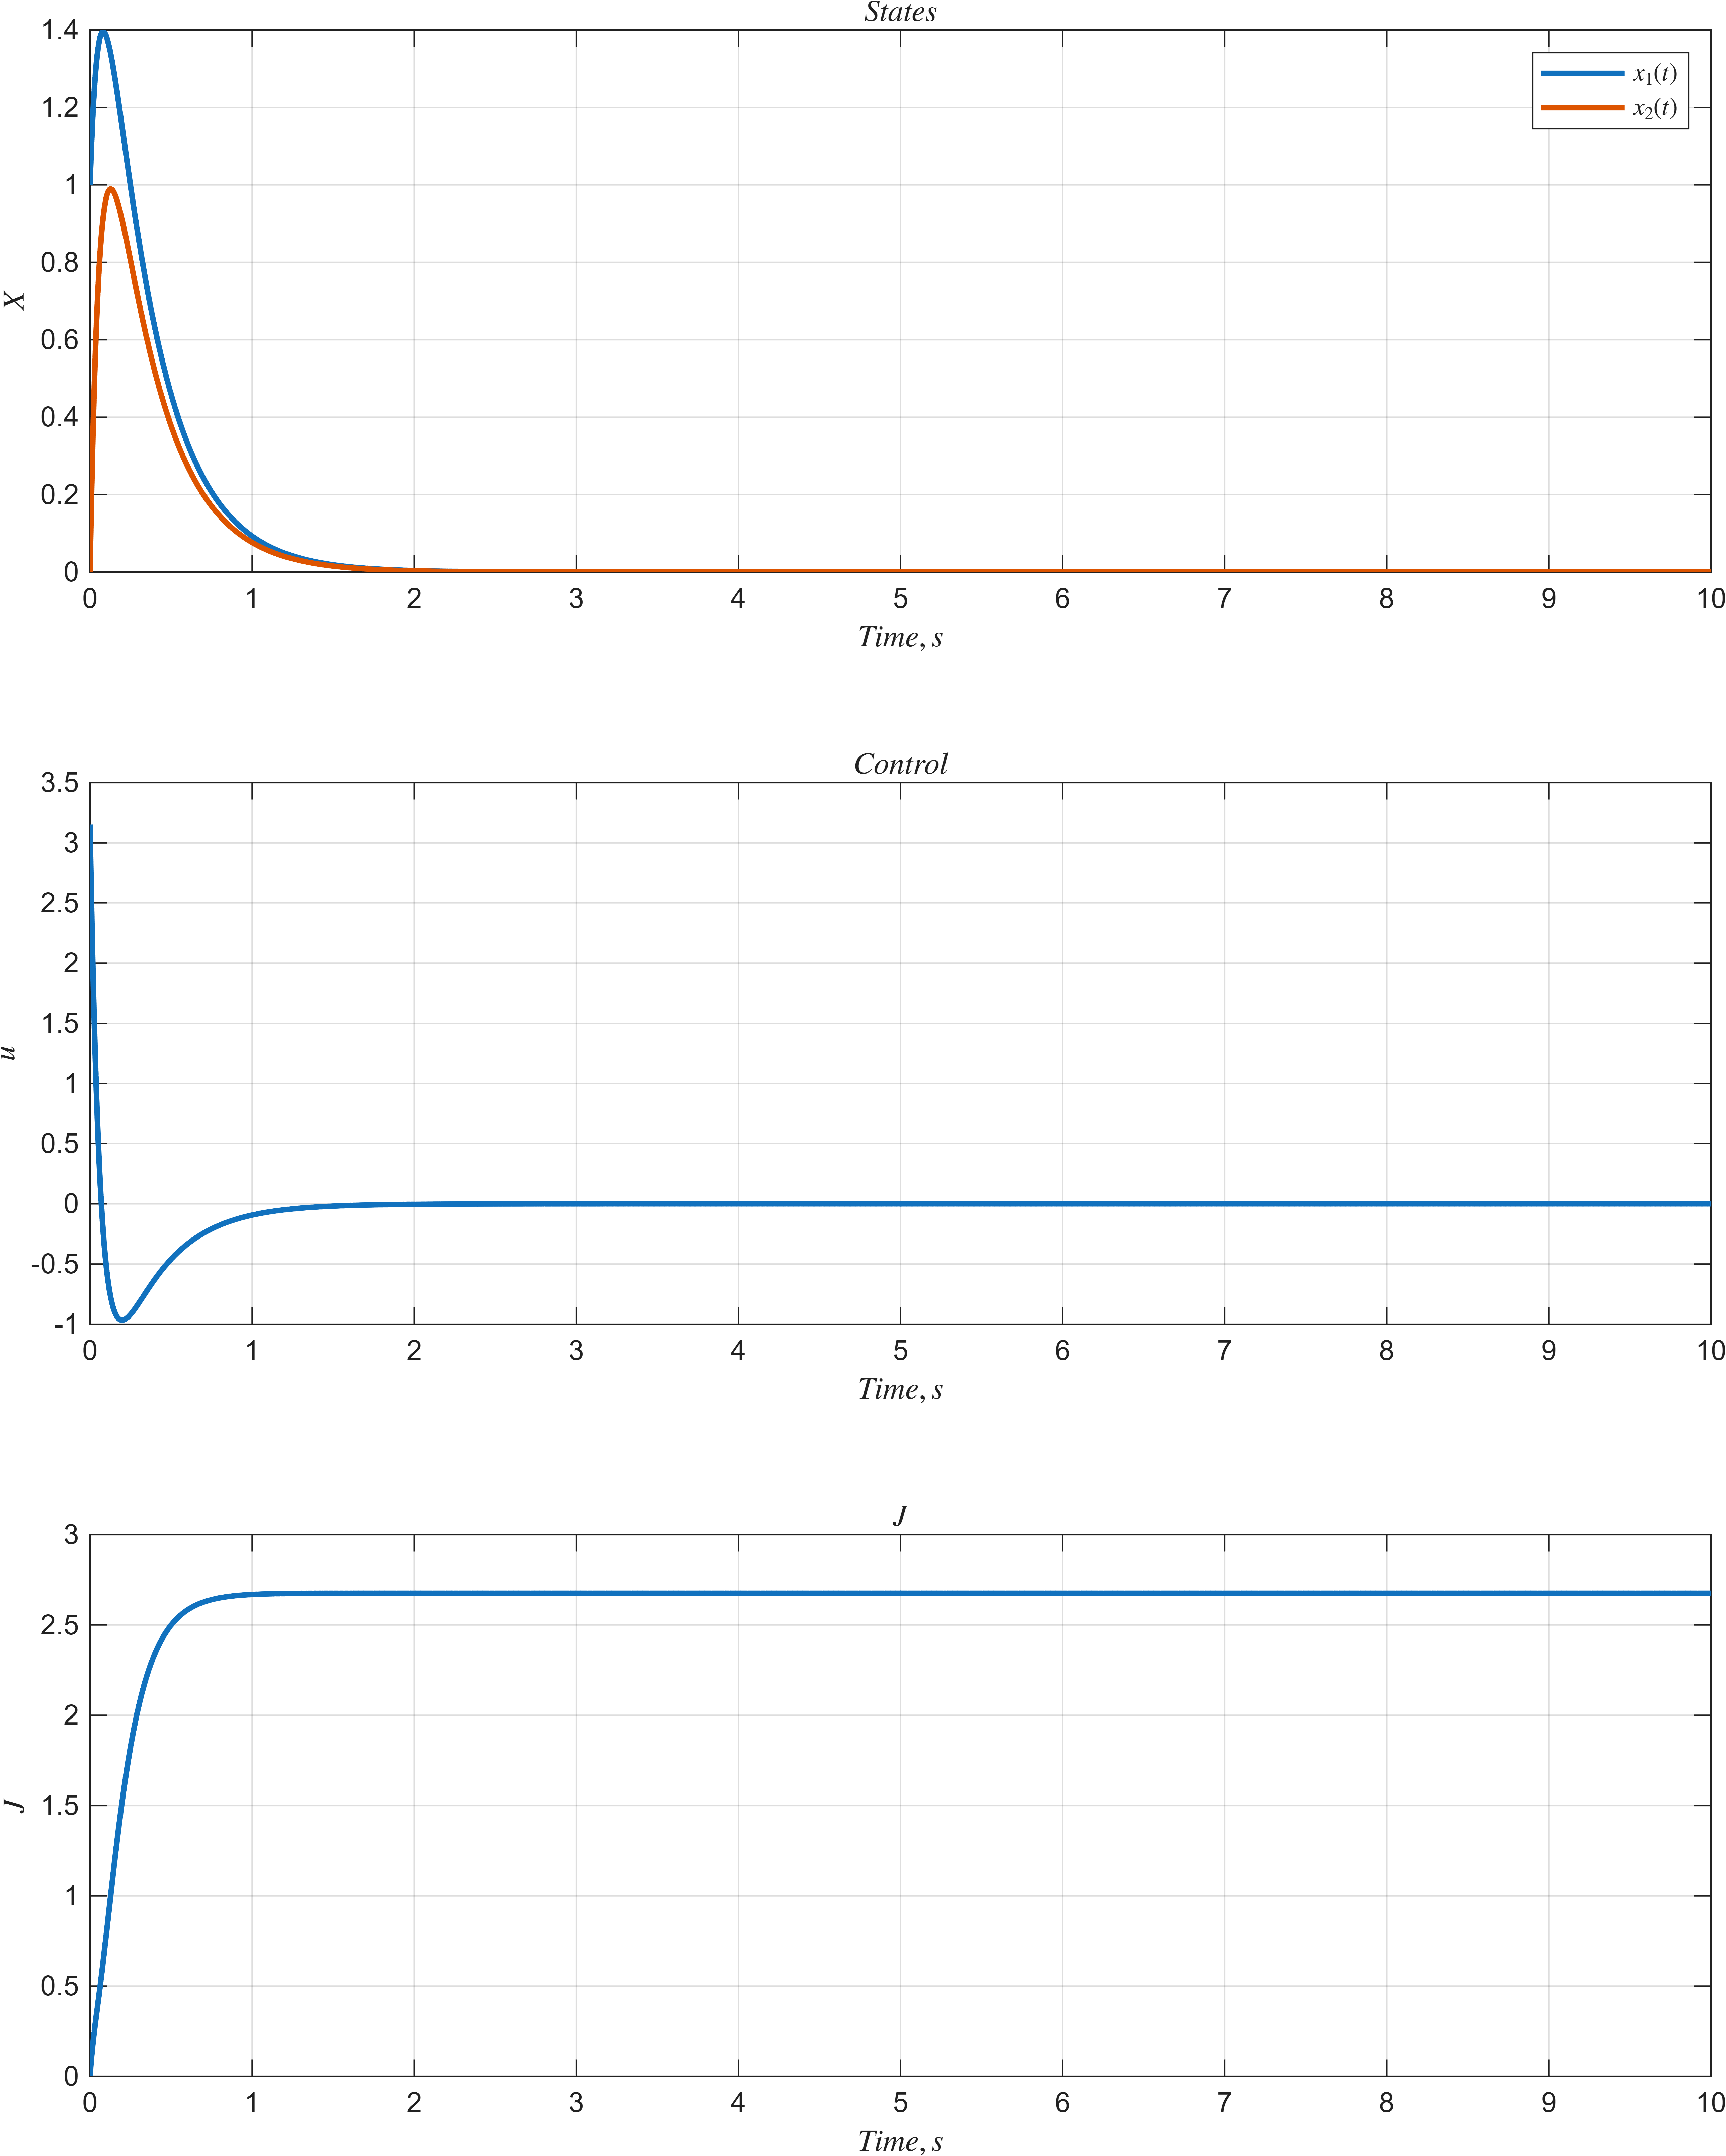
\includegraphics[width=0.9\textwidth]{images/task2.png}
    \caption{Результаты моделирования замкнутой системы}
    \label{fig:task2}
\end{figure}

Из полученных графиков видно, что обе компоненты
вектора состояния $x_1(t)$ и $x_2(t)$ стремятся
к нулю, что подтверждает асимптотическую
устойчивость замкнутой системы.

Управляющее воздействие $u(t)$ также стремится
к нулю, а критерий качества $J(t)$ монотонно
возрастает и выходит на установившееся значение
\[
J_{\mathrm{уст}}\approx2{,}6761
\]

Теоретическое минимальное значение критерия качества
определяется выражением
\[
J^*=\bm x^{T}(0)P\bm x(0)
\]

С учётом начальных условий получаем
\[
\begin{aligned}
J^*
&=
\begin{pmatrix}1&0\end{pmatrix}
\begin{pmatrix}
2{,}676107&-1{,}731905\\
-1{,}731905&1{,}496937
\end{pmatrix}
\begin{pmatrix}1\\0\end{pmatrix}
\\[2mm]
&=p_{11}\approx2{,}676107
\end{aligned}
\]

Таким образом
\[
J_{\mathrm{уст}}\approx J^*
\]

Полученное при моделировании значение критерия
качества совпадает с теоретическим, что подтверждает
корректность расчёта оптимального регулятора.


\section{Исследование изменения коэффициентов регулятора}

Изменим коэффициенты оптимального регулятора
\[
K=\begin{pmatrix}
-3{,}150813&5{,}047877
\end{pmatrix}
\]

Примем новые значения
\[
\widetilde K=\begin{pmatrix}-3&5\end{pmatrix}
\]

Отклонение коэффициентов составляет
\[
\Delta K=\widetilde K-K
=\begin{pmatrix}
0{,}150813&-0{,}047877
\end{pmatrix}
\]

Проверим устойчивость замкнутой системы с изменённым регулятором
\[
\dot{\bm x}=(A-\bm b\widetilde K)\bm x
\]

Матрица замкнутой системы
\[
\begin{aligned}
\widetilde F
&=A-\bm b\widetilde K\\
&=
\begin{pmatrix}
0&1\\
-2&9
\end{pmatrix}
-
\begin{pmatrix}4\\8\end{pmatrix}
\begin{pmatrix}-3&5\end{pmatrix}\\
&=
\begin{pmatrix}
12&-19\\
22&-31
\end{pmatrix}
\end{aligned}
\]

Для асимптотической устойчивости системы второго порядка необходимо и достаточно выполнения условий
\[
\operatorname{tr}\widetilde F<0,
\qquad
\det\widetilde F>0
\]

Вычислим след и определитель
\[
\operatorname{tr}\widetilde F=12-31=-19<0
\]

\[
\det\widetilde F
=12\cdot(-31)-(-19)\cdot22=46>0
\]

Характеристическое уравнение имеет вид
\[
\det(\lambda I-\widetilde F)=0
\]

\[
\lambda^2+19\lambda+46=0
\]

Собственные значения матрицы
\[
\lambda_{1,2}=\frac{-19\pm\sqrt{177}}{2}
\]

\[
\begin{aligned}
\lambda_1&\approx-2{,}847933\\
\lambda_2&\approx-16{,}152067
\end{aligned}
\]

Оба собственных значения отрицательны, следовательно, замкнутая система сохраняет асимптотическую устойчивость.

Новый закон управления имеет вид
\[
\widetilde u(t)=3x_1(t)-5x_2(t)
\]

Проведём моделирование с изменёнными коэффициентами при тех же начальных условиях и времени моделирования
\[
\bm x(0)=
\begin{pmatrix}1\\0\end{pmatrix},
\qquad t\in[0,10]
\]

Для определения установившегося значения критерия качества изменённого регулятора используем уравнение Ляпунова
\[
\widetilde F^TS+S\widetilde F+
Q+r\widetilde K^T\widetilde K=0
\]

Представим матрицу $S$ в виде
\[
S=\begin{pmatrix}
s_{11}&s_{12}\\
s_{12}&s_{22}
\end{pmatrix}
\]

Поскольку
\[
Q+r\widetilde K^T\widetilde K
=
\begin{pmatrix}
12&-15\\
-15&27
\end{pmatrix}
\]

получаем систему уравнений
\[
\begin{cases}
24s_{11}+44s_{12}+12=0\\
-19s_{11}-19s_{12}+22s_{22}-15=0\\
-38s_{12}-62s_{22}+27=0
\end{cases}
\]

Решая систему, находим
\[
S=
\begin{pmatrix}
\dfrac{51}{19}&-\dfrac{33}{19}\\[2mm]
-\dfrac{33}{19}&\dfrac{3}{2}
\end{pmatrix}
\]

Установившееся значение критерия качества для изменённого регулятора
\[
\begin{aligned}
\widetilde J_{\mathrm{уст}}
&=\bm x^T(0)S\bm x(0)\\
&=
\begin{pmatrix}1&0\end{pmatrix}
S\begin{pmatrix}1\\0\end{pmatrix}\\
&=\frac{51}{19}\approx2{,}684211
\end{aligned}
\]

Для оптимального регулятора ранее получено
\[
J^*\approx2{,}676107
\]

Разность значений критерия качества
\[
\begin{aligned}
\Delta J
&=\widetilde J_{\mathrm{уст}}-J^*\\
&\approx2{,}684211-2{,}676107\\
&\approx0{,}008103
\end{aligned}
\]

Относительное увеличение критерия качества
\[
\delta_J=
\frac{\Delta J}{J^*}\cdot100\%
\approx0{,}303\%
\]

Результаты моделирования исходного и изменённого регуляторов представлены на рисунке \ref{fig:task3}.

\begin{figure}[htbp]
    \centering
    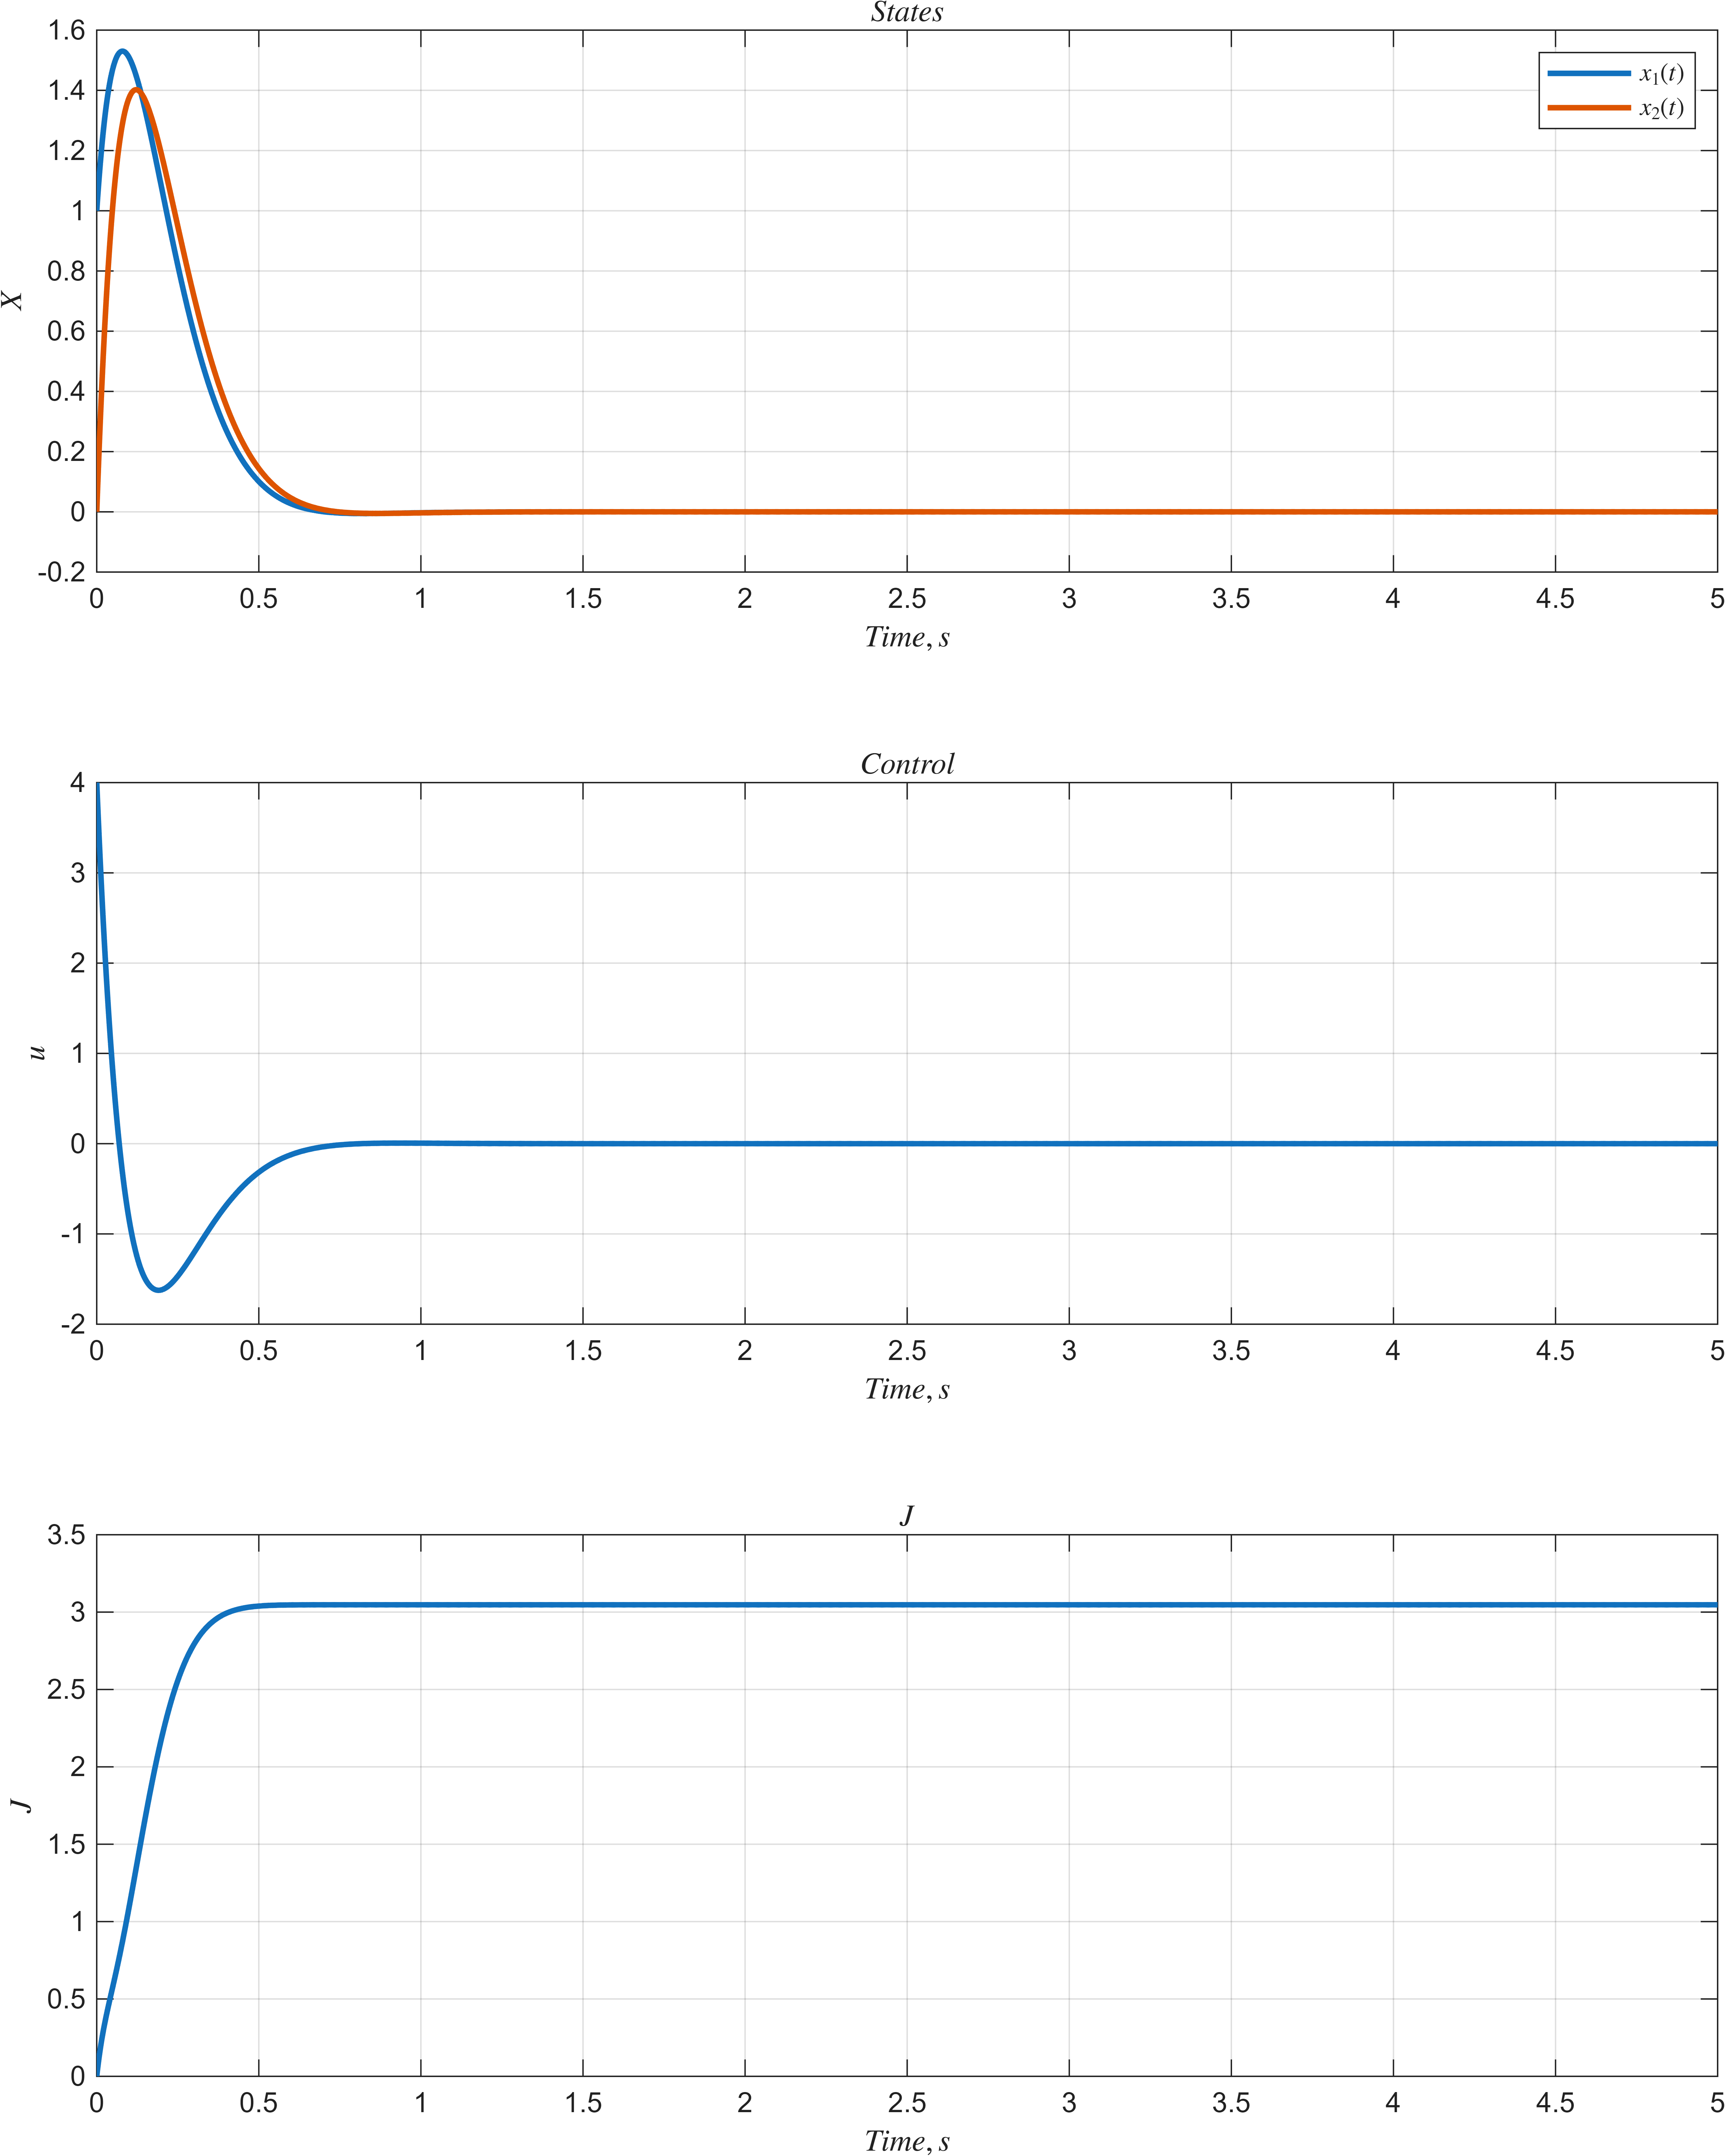
\includegraphics[width=0.9\textwidth]{images/task3.png}
    \caption{Сравнение результатов моделирования исходного и изменённого регуляторов}
    \label{fig:task3}
\end{figure}

Изменение коэффициентов регулятора не привело к потере устойчивости замкнутой системы. Обе компоненты вектора состояния и управляющее воздействие стремятся к нулю.

При этом установившееся значение критерия качества увеличилось на $0{,}303\%$. Следовательно, изменённый регулятор сохраняет устойчивость системы, но уступает исходному оптимальному регулятору по критерию качества.
